\documentclass[a4paper]{book}
\usepackage{a4wide}
\usepackage{makeidx}
\usepackage{fancyhdr}
\usepackage{graphicx}
\usepackage{multicol}
\usepackage{float}
\usepackage{listings}
\usepackage{color}
\usepackage{textcomp}
\usepackage{alltt}
\usepackage{times}
\usepackage[utf8]{inputenc}
\usepackage{doxygen}
\lstset{language=C++,inputencoding=utf8,basicstyle=\footnotesize,breaklines=true,breakatwhitespace=true,tabsize=1,numbers=left }
\makeindex
\setcounter{tocdepth}{3}
\renewcommand{\footrulewidth}{0.4pt}
\begin{document}
\begin{titlepage}
\vspace*{7cm}
\begin{center}
{\Large Reference Manual}\\
\vspace*{1cm}
{\large Generated by Doxygen 1.5.9}\\
\vspace*{0.5cm}
{\small Thu Jul 23 12:35:44 2009}\\
\end{center}
\end{titlepage}
\clearemptydoublepage
\pagenumbering{roman}
\tableofcontents
\clearemptydoublepage
\pagenumbering{arabic}
\chapter{Class Index}
\section{Class Hierarchy}
This inheritance list is sorted roughly, but not completely, alphabetically:\begin{CompactList}
\item \contentsline{section}{ExampleApplication}{\pageref{class_example_application}}{}
\begin{CompactList}
\item \contentsline{section}{PVApplication}{\pageref{class_p_v_application}}{}
\end{CompactList}
\item \contentsline{section}{ExampleFrameListener}{\pageref{class_example_frame_listener}}{}
\begin{CompactList}
\item \contentsline{section}{PVFrameListener}{\pageref{class_p_v_frame_listener}}{}
\end{CompactList}
\item \contentsline{section}{KeyListener}{\pageref{class_o_i_s_1_1_key_listener}}{}
\begin{CompactList}
\item \contentsline{section}{PVFrameListener}{\pageref{class_p_v_frame_listener}}{}
\end{CompactList}
\item \contentsline{section}{PVNode}{\pageref{class_p_v_node}}{}
\begin{CompactList}
\item \contentsline{section}{PVBall}{\pageref{class_p_v_ball}}{}
\end{CompactList}
\item \contentsline{section}{PVPhysics}{\pageref{class_p_v_physics}}{}
\item \contentsline{section}{PVTimer}{\pageref{class_p_v_timer}}{}
\end{CompactList}

\chapter{Class Index}
\section{Class List}
Here are the classes, structs, unions and interfaces with brief descriptions:\begin{CompactList}
\item\contentsline{section}{{\bf ExampleApplication} }{\pageref{class_example_application}}{}
\item\contentsline{section}{{\bf ExampleFrameListener} }{\pageref{class_example_frame_listener}}{}
\item\contentsline{section}{{\bf KeyListener} }{\pageref{class_o_i_s_1_1_key_listener}}{}
\item\contentsline{section}{{\bf PVApplication} }{\pageref{class_p_v_application}}{}
\item\contentsline{section}{{\bf PVBall} }{\pageref{class_p_v_ball}}{}
\item\contentsline{section}{{\bf PVFrameListener} }{\pageref{class_p_v_frame_listener}}{}
\item\contentsline{section}{{\bf PVNode} }{\pageref{class_p_v_node}}{}
\item\contentsline{section}{{\bf PVPhysics} }{\pageref{class_p_v_physics}}{}
\item\contentsline{section}{{\bf PVTimer} }{\pageref{class_p_v_timer}}{}
\end{CompactList}

\chapter{Class Documentation}
\section{ExampleApplication Class Reference}
\label{class_example_application}\index{ExampleApplication@{ExampleApplication}}
Inherited by {\bf PVApplication}.



The documentation for this class was generated from the following file:\begin{CompactItemize}
\item 
BallApp.h\end{CompactItemize}

\section{ExampleFrameListener Class Reference}
\label{class_example_frame_listener}\index{ExampleFrameListener@{ExampleFrameListener}}
Inherited by {\bf PVFrameListener}.



The documentation for this class was generated from the following file:\begin{CompactItemize}
\item 
BallApp.h\end{CompactItemize}

\section{KeyListener Class Reference}
\label{class_o_i_s_1_1_key_listener}\index{OIS::KeyListener@{OIS::KeyListener}}
Inherited by {\bf PVFrameListener}.



The documentation for this class was generated from the following file:\begin{CompactItemize}
\item 
BallApp.h\end{CompactItemize}

\section{PVApplication Class Reference}
\label{class_p_v_application}\index{PVApplication@{PVApplication}}
Inherits {\bf ExampleApplication}.

Collaboration diagram for PVApplication:\nopagebreak
\begin{figure}[H]
\begin{center}
\leavevmode
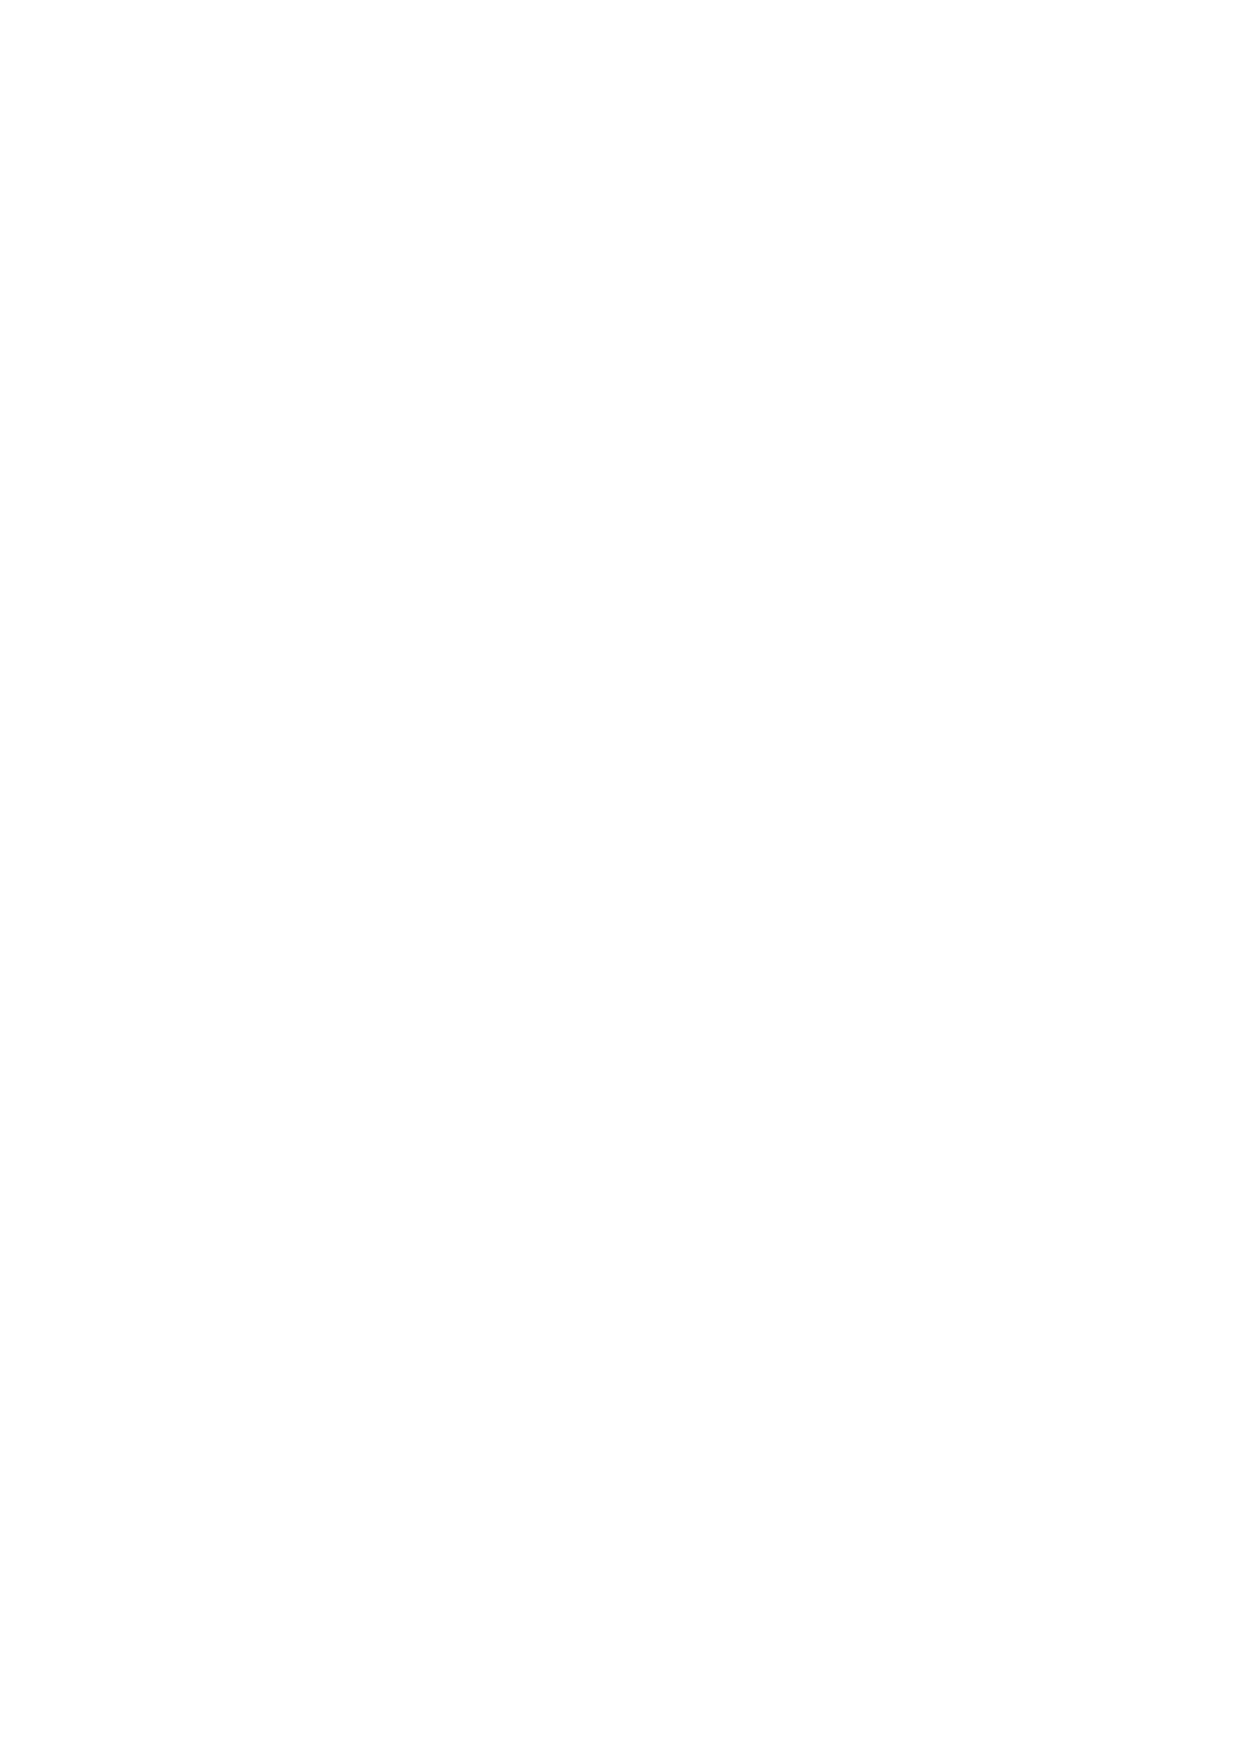
\includegraphics[width=44pt]{class_p_v_application__coll__graph}
\end{center}
\end{figure}
\subsection*{Public Member Functions}
\begin{CompactItemize}
\item 
{\bf PVApplication} ()
\item 
{\bf $\sim$PVApplication} ()
\item 
void {\bf clearAllBalls} ()
\item 
void {\bf createBalls} ()
\end{CompactItemize}
\subsection*{Public Attributes}
\begin{CompactItemize}
\item 
int {\bf m\_\-numberOfBalls}
\end{CompactItemize}
\subsection*{Protected Member Functions}
\begin{CompactItemize}
\item 
void {\bf createCamera} (void)
\item 
void {\bf createViewports} (void)
\item 
void {\bf createScene} (void)
\item 
void {\bf createFrameListener} (void)
\end{CompactItemize}
\subsection*{Protected Attributes}
\begin{CompactItemize}
\item 
std::map$<$ std::string, {\bf PVNode} $\ast$ $>$ {\bf m\_\-objectMap}
\item 
std::vector$<$ {\bf PVNode} $\ast$ $>$ {\bf m\_\-balls}
\end{CompactItemize}


\subsection{Constructor \& Destructor Documentation}
\index{PVApplication@{PVApplication}!PVApplication@{PVApplication}}
\index{PVApplication@{PVApplication}!PVApplication@{PVApplication}}
\subsubsection[{PVApplication}]{\setlength{\rightskip}{0pt plus 5cm}PVApplication::PVApplication ()}\label{class_p_v_application_621fc385e12d3823366490cb93ebc9a9}


Constructor. 

\index{PVApplication@{PVApplication}!$\sim$PVApplication@{$\sim$PVApplication}}
\index{$\sim$PVApplication@{$\sim$PVApplication}!PVApplication@{PVApplication}}
\subsubsection[{$\sim$PVApplication}]{\setlength{\rightskip}{0pt plus 5cm}PVApplication::$\sim$PVApplication ()}\label{class_p_v_application_3d86091863293b76b98694cafc7d9591}


Destructor. 



\subsection{Member Function Documentation}
\index{PVApplication@{PVApplication}!clearAllBalls@{clearAllBalls}}
\index{clearAllBalls@{clearAllBalls}!PVApplication@{PVApplication}}
\subsubsection[{clearAllBalls}]{\setlength{\rightskip}{0pt plus 5cm}void PVApplication::clearAllBalls ()}\label{class_p_v_application_4e2bf04991d47db48f4b8ae7a7f261fc}


funtkion for deleting all balls in the scene. 

\index{PVApplication@{PVApplication}!createBalls@{createBalls}}
\index{createBalls@{createBalls}!PVApplication@{PVApplication}}
\subsubsection[{createBalls}]{\setlength{\rightskip}{0pt plus 5cm}void PVApplication::createBalls ()}\label{class_p_v_application_8fb729cf23610211b98f202d9334595f}


creates a vector with balls. 

\index{PVApplication@{PVApplication}!createCamera@{createCamera}}
\index{createCamera@{createCamera}!PVApplication@{PVApplication}}
\subsubsection[{createCamera}]{\setlength{\rightskip}{0pt plus 5cm}void PVApplication::createCamera (void)\hspace{0.3cm}{\tt  [protected]}}\label{class_p_v_application_81f6bb4306c063fd2fb2df9753c33d3a}


Set camera settings. 

\index{PVApplication@{PVApplication}!createViewports@{createViewports}}
\index{createViewports@{createViewports}!PVApplication@{PVApplication}}
\subsubsection[{createViewports}]{\setlength{\rightskip}{0pt plus 5cm}void PVApplication::createViewports (void)\hspace{0.3cm}{\tt  [protected]}}\label{class_p_v_application_c80a64cba5a004cf50b8373832a0571c}


Set viewport settings. 

\index{PVApplication@{PVApplication}!createScene@{createScene}}
\index{createScene@{createScene}!PVApplication@{PVApplication}}
\subsubsection[{createScene}]{\setlength{\rightskip}{0pt plus 5cm}void PVApplication::createScene (void)\hspace{0.3cm}{\tt  [protected]}}\label{class_p_v_application_d06164df52925a385a306e5b3bf9c68c}


Create scene. 

\index{PVApplication@{PVApplication}!createFrameListener@{createFrameListener}}
\index{createFrameListener@{createFrameListener}!PVApplication@{PVApplication}}
\subsubsection[{createFrameListener}]{\setlength{\rightskip}{0pt plus 5cm}void PVApplication::createFrameListener (void)\hspace{0.3cm}{\tt  [protected]}}\label{class_p_v_application_f3c0a1a5ba0863381dc566387d5cea14}


Create Framelistener. 



\subsection{Member Data Documentation}
\index{PVApplication@{PVApplication}!m\_\-numberOfBalls@{m\_\-numberOfBalls}}
\index{m\_\-numberOfBalls@{m\_\-numberOfBalls}!PVApplication@{PVApplication}}
\subsubsection[{m\_\-numberOfBalls}]{\setlength{\rightskip}{0pt plus 5cm}int {\bf PVApplication::m\_\-numberOfBalls}}\label{class_p_v_application_a21695e21355042d06746c1b4dc921f8}


max number of balls. 

\index{PVApplication@{PVApplication}!m\_\-objectMap@{m\_\-objectMap}}
\index{m\_\-objectMap@{m\_\-objectMap}!PVApplication@{PVApplication}}
\subsubsection[{m\_\-objectMap}]{\setlength{\rightskip}{0pt plus 5cm}std::map$<$std::string, {\bf PVNode}$\ast$$>$ {\bf PVApplication::m\_\-objectMap}\hspace{0.3cm}{\tt  [protected]}}\label{class_p_v_application_391465236459221a65ba4361fa306db3}


map with scene objects. 

\index{PVApplication@{PVApplication}!m\_\-balls@{m\_\-balls}}
\index{m\_\-balls@{m\_\-balls}!PVApplication@{PVApplication}}
\subsubsection[{m\_\-balls}]{\setlength{\rightskip}{0pt plus 5cm}std::vector$<${\bf PVNode}$\ast$$>$ {\bf PVApplication::m\_\-balls}\hspace{0.3cm}{\tt  [protected]}}\label{class_p_v_application_80794ff58204fb039f2aa58ed0d157a1}


vector with balls. 



The documentation for this class was generated from the following files:\begin{CompactItemize}
\item 
BallApp.h\item 
BallApp.cpp\item 
main.cpp\end{CompactItemize}

\section{PVBall Class Reference}
\label{class_p_v_ball}\index{PVBall@{PVBall}}
Inherits {\bf PVNode}.

Collaboration diagram for PVBall:\nopagebreak
\begin{figure}[H]
\begin{center}
\leavevmode
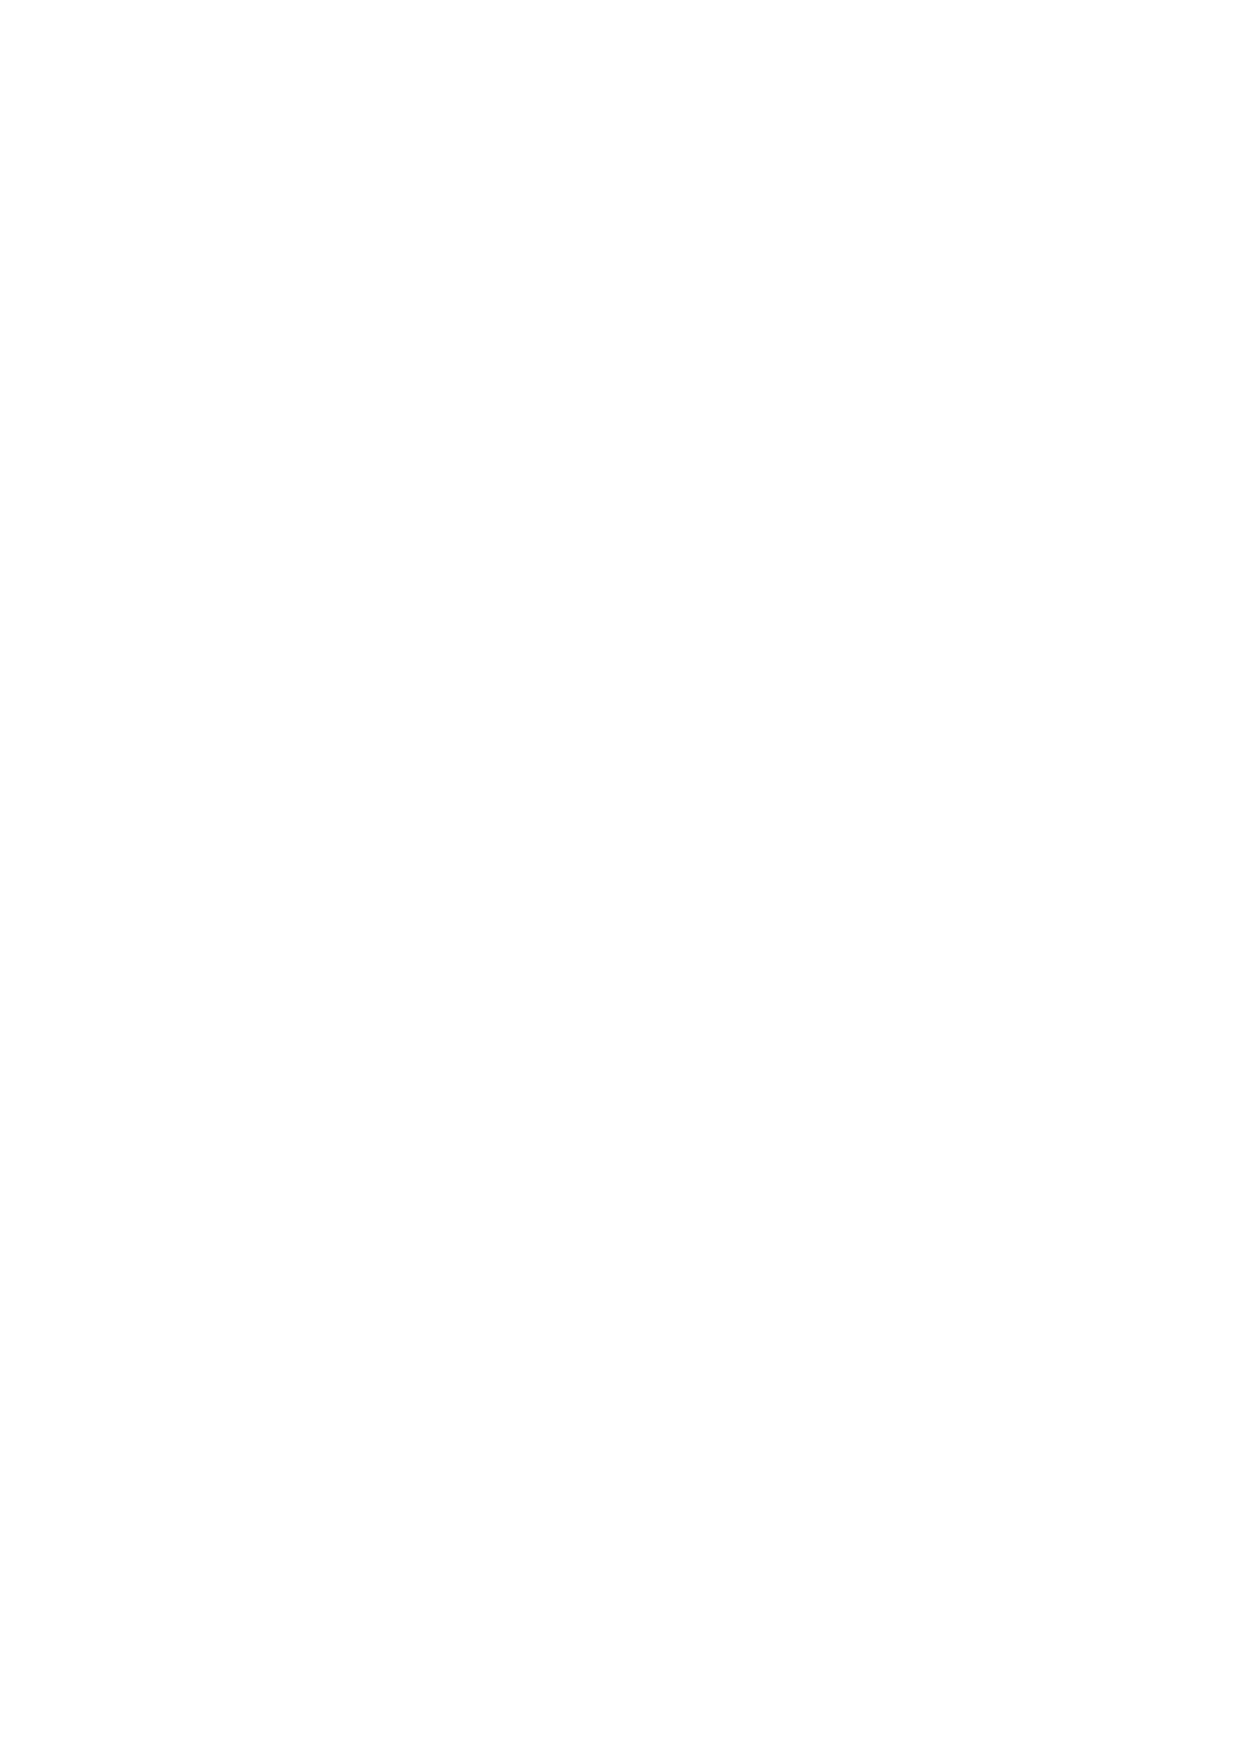
\includegraphics[width=44pt]{class_p_v_ball__coll__graph}
\end{center}
\end{figure}
\subsection*{Public Member Functions}
\begin{CompactItemize}
\item 
{\bf PVBall} ()
\item 
{\bf PVBall} (SceneNode $\ast$node, Entity $\ast$entity)
\item 
virtual {\bf $\sim$PVBall} ()
\item 
bool {\bf intersect} ()
\item 
int {\bf getId} ()
\item 
void {\bf setBallId} (int id)
\end{CompactItemize}
\subsection*{Static Public Member Functions}
\begin{CompactItemize}
\item 
static int {\bf getBallCount} ()
\end{CompactItemize}


\subsection{Constructor \& Destructor Documentation}
\index{PVBall@{PVBall}!PVBall@{PVBall}}
\index{PVBall@{PVBall}!PVBall@{PVBall}}
\subsubsection[{PVBall}]{\setlength{\rightskip}{0pt plus 5cm}PVBall::PVBall ()}\label{class_p_v_ball_86502630f0f62a9a51f7c51bf9519409}


\index{PVBall@{PVBall}!PVBall@{PVBall}}
\index{PVBall@{PVBall}!PVBall@{PVBall}}
\subsubsection[{PVBall}]{\setlength{\rightskip}{0pt plus 5cm}PVBall::PVBall (SceneNode $\ast$ {\em node}, \/  Entity $\ast$ {\em entity})}\label{class_p_v_ball_12ef7c87d000beae278975193872de49}


\index{PVBall@{PVBall}!$\sim$PVBall@{$\sim$PVBall}}
\index{$\sim$PVBall@{$\sim$PVBall}!PVBall@{PVBall}}
\subsubsection[{$\sim$PVBall}]{\setlength{\rightskip}{0pt plus 5cm}PVBall::$\sim$PVBall ()\hspace{0.3cm}{\tt  [virtual]}}\label{class_p_v_ball_a00806c0b3ea8703fd8f3882baa75a7d}




\subsection{Member Function Documentation}
\index{PVBall@{PVBall}!intersect@{intersect}}
\index{intersect@{intersect}!PVBall@{PVBall}}
\subsubsection[{intersect}]{\setlength{\rightskip}{0pt plus 5cm}bool PVBall::intersect ()}\label{class_p_v_ball_f9a225f53d94a8bf804e260d10ec34ee}


\index{PVBall@{PVBall}!getId@{getId}}
\index{getId@{getId}!PVBall@{PVBall}}
\subsubsection[{getId}]{\setlength{\rightskip}{0pt plus 5cm}int PVBall::getId ()}\label{class_p_v_ball_ba4d460f5a7d8e3741e9ab2f438157ca}


\index{PVBall@{PVBall}!setBallId@{setBallId}}
\index{setBallId@{setBallId}!PVBall@{PVBall}}
\subsubsection[{setBallId}]{\setlength{\rightskip}{0pt plus 5cm}void PVBall::setBallId (int {\em id})}\label{class_p_v_ball_5302c6790e1ac845b98c93b44d2dc5e4}


\index{PVBall@{PVBall}!getBallCount@{getBallCount}}
\index{getBallCount@{getBallCount}!PVBall@{PVBall}}
\subsubsection[{getBallCount}]{\setlength{\rightskip}{0pt plus 5cm}static int PVBall::getBallCount ()\hspace{0.3cm}{\tt  [static]}}\label{class_p_v_ball_7eb5352c9f20854605387107be0552e3}




The documentation for this class was generated from the following files:\begin{CompactItemize}
\item 
PVBall.h\item 
PVBall.cpp\end{CompactItemize}

\section{PVFrameListener Class Reference}
\label{class_p_v_frame_listener}\index{PVFrameListener@{PVFrameListener}}
Inherits {\bf ExampleFrameListener}, and {\bf OIS::KeyListener}.

Collaboration diagram for PVFrameListener:\nopagebreak
\begin{figure}[H]
\begin{center}
\leavevmode
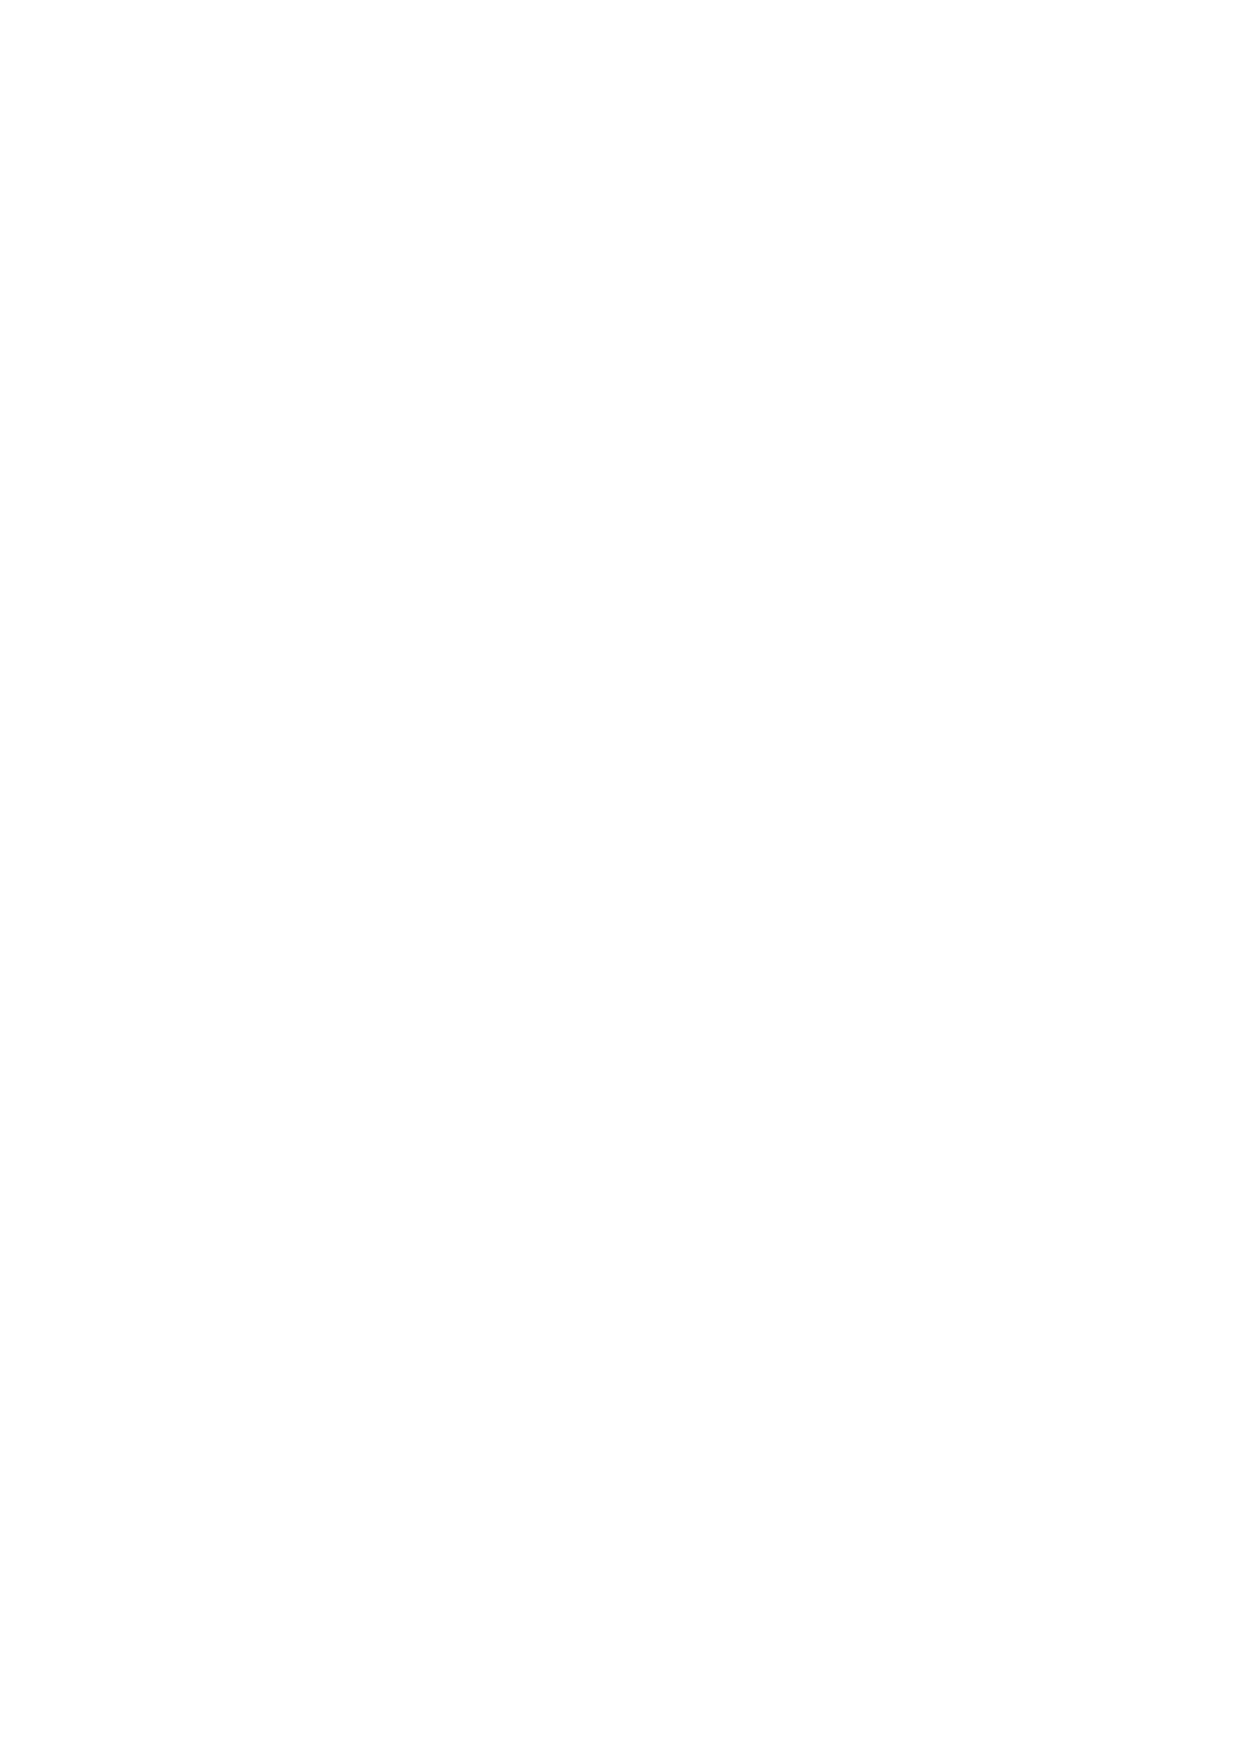
\includegraphics[width=44pt]{class_p_v_frame_listener__coll__graph}
\end{center}
\end{figure}
\subsection*{Public Member Functions}
\begin{CompactItemize}
\item 
{\bf PVFrameListener} (RenderWindow $\ast$win, Camera $\ast$cam, SceneManager $\ast$sceneMgr, std::map$<$ std::string, {\bf PVNode} $\ast$ $>$ \&objectMap, std::vector$<$ {\bf PVNode} $\ast$ $>$ \&balls, {\bf PVApplication} $\ast$app)
\item 
bool {\bf frameStarted} (const FrameEvent \&evt)
\item 
bool {\bf keyPressed} (const OIS::KeyEvent \&arg)
\item 
bool {\bf keyReleased} (const OIS::KeyEvent \&arg)
\end{CompactItemize}
\subsection*{Protected Attributes}
\begin{CompactItemize}
\item 
bool {\bf mMouseDownBool}
\item 
Real {\bf mToggle}
\item 
Real {\bf mRotate}
\item 
Real {\bf mMove}
\item 
SceneManager $\ast$ {\bf mSceneMgr}
\item 
SceneNode $\ast$ {\bf mCamNode}
\item 
bool {\bf mContinue}
\end{CompactItemize}


\subsection{Constructor \& Destructor Documentation}
\index{PVFrameListener@{PVFrameListener}!PVFrameListener@{PVFrameListener}}
\index{PVFrameListener@{PVFrameListener}!PVFrameListener@{PVFrameListener}}
\subsubsection[{PVFrameListener}]{\setlength{\rightskip}{0pt plus 5cm}PVFrameListener::PVFrameListener (RenderWindow $\ast$ {\em win}, \/  Camera $\ast$ {\em cam}, \/  SceneManager $\ast$ {\em sceneMgr}, \/  std::map$<$ std::string, {\bf PVNode} $\ast$ $>$ \& {\em objectMap}, \/  std::vector$<$ {\bf PVNode} $\ast$ $>$ \& {\em balls}, \/  {\bf PVApplication} $\ast$ {\em app})}\label{class_p_v_frame_listener_c9505ee626a8e6dccf582f909c988857}


Constructor. 

\begin{Desc}
\item[Parameters:]
\begin{description}
\item[{\em win}]the window for rendering. \item[{\em sceneMgr}]the scene manager. \item[{\em objectMap}]a map with PVNodes. \item[{\em app}]an instance of \doxyref{PVApplication}{p.}{class_p_v_application}. \end{description}
\end{Desc}


\subsection{Member Function Documentation}
\index{PVFrameListener@{PVFrameListener}!frameStarted@{frameStarted}}
\index{frameStarted@{frameStarted}!PVFrameListener@{PVFrameListener}}
\subsubsection[{frameStarted}]{\setlength{\rightskip}{0pt plus 5cm}bool PVFrameListener::frameStarted (const FrameEvent \& {\em evt})}\label{class_p_v_frame_listener_aa60d3ba4840a661c598914a4134af56}


Ogre callback funktion for simulation. 

\begin{Desc}
\item[Parameters:]
\begin{description}
\item[{\em \&evt}]an event. \end{description}
\end{Desc}
\index{PVFrameListener@{PVFrameListener}!keyPressed@{keyPressed}}
\index{keyPressed@{keyPressed}!PVFrameListener@{PVFrameListener}}
\subsubsection[{keyPressed}]{\setlength{\rightskip}{0pt plus 5cm}bool PVFrameListener::keyPressed (const OIS::KeyEvent \& {\em arg})}\label{class_p_v_frame_listener_af53be6906b2b74c293a57b7a3f7254b}


callback funktion for pressing key. 

\begin{Desc}
\item[Parameters:]
\begin{description}
\item[{\em \&arg}]a key event. \end{description}
\end{Desc}
\index{PVFrameListener@{PVFrameListener}!keyReleased@{keyReleased}}
\index{keyReleased@{keyReleased}!PVFrameListener@{PVFrameListener}}
\subsubsection[{keyReleased}]{\setlength{\rightskip}{0pt plus 5cm}bool PVFrameListener::keyReleased (const OIS::KeyEvent \& {\em arg})}\label{class_p_v_frame_listener_63896b4b8aed99c89e0bb54a33db7411}


callback funktion for releasing a key. 

\begin{Desc}
\item[Parameters:]
\begin{description}
\item[{\em \&arg}]a key event. \end{description}
\end{Desc}


\subsection{Member Data Documentation}
\index{PVFrameListener@{PVFrameListener}!mMouseDownBool@{mMouseDownBool}}
\index{mMouseDownBool@{mMouseDownBool}!PVFrameListener@{PVFrameListener}}
\subsubsection[{mMouseDownBool}]{\setlength{\rightskip}{0pt plus 5cm}bool {\bf PVFrameListener::mMouseDownBool}\hspace{0.3cm}{\tt  [protected]}}\label{class_p_v_frame_listener_41f96e4117faec7561bee96517203dff}


Whether or not the left mouse button was down last frame. 

\index{PVFrameListener@{PVFrameListener}!mToggle@{mToggle}}
\index{mToggle@{mToggle}!PVFrameListener@{PVFrameListener}}
\subsubsection[{mToggle}]{\setlength{\rightskip}{0pt plus 5cm}Real {\bf PVFrameListener::mToggle}\hspace{0.3cm}{\tt  [protected]}}\label{class_p_v_frame_listener_81242d0a61756621f5eaf6259e25e8d9}


The time left until next toggle. 

\index{PVFrameListener@{PVFrameListener}!mRotate@{mRotate}}
\index{mRotate@{mRotate}!PVFrameListener@{PVFrameListener}}
\subsubsection[{mRotate}]{\setlength{\rightskip}{0pt plus 5cm}Real {\bf PVFrameListener::mRotate}\hspace{0.3cm}{\tt  [protected]}}\label{class_p_v_frame_listener_433d7a46809228e5c37086e5590b54b0}


The rotate constant. 

\index{PVFrameListener@{PVFrameListener}!mMove@{mMove}}
\index{mMove@{mMove}!PVFrameListener@{PVFrameListener}}
\subsubsection[{mMove}]{\setlength{\rightskip}{0pt plus 5cm}Real {\bf PVFrameListener::mMove}\hspace{0.3cm}{\tt  [protected]}}\label{class_p_v_frame_listener_408e19582e839e8578e5f15b430a6fa4}


The movement constant. 

\index{PVFrameListener@{PVFrameListener}!mSceneMgr@{mSceneMgr}}
\index{mSceneMgr@{mSceneMgr}!PVFrameListener@{PVFrameListener}}
\subsubsection[{mSceneMgr}]{\setlength{\rightskip}{0pt plus 5cm}SceneManager$\ast$ {\bf PVFrameListener::mSceneMgr}\hspace{0.3cm}{\tt  [protected]}}\label{class_p_v_frame_listener_8cd3d9e70c8495b2b2d90ca1b16f39cc}


The current SceneManager. 

\index{PVFrameListener@{PVFrameListener}!mCamNode@{mCamNode}}
\index{mCamNode@{mCamNode}!PVFrameListener@{PVFrameListener}}
\subsubsection[{mCamNode}]{\setlength{\rightskip}{0pt plus 5cm}SceneNode$\ast$ {\bf PVFrameListener::mCamNode}\hspace{0.3cm}{\tt  [protected]}}\label{class_p_v_frame_listener_c0e9f972099daf74487771d11e9ae4fb}


The SceneNode the camera is currently attached to. 

\index{PVFrameListener@{PVFrameListener}!mContinue@{mContinue}}
\index{mContinue@{mContinue}!PVFrameListener@{PVFrameListener}}
\subsubsection[{mContinue}]{\setlength{\rightskip}{0pt plus 5cm}bool {\bf PVFrameListener::mContinue}\hspace{0.3cm}{\tt  [protected]}}\label{class_p_v_frame_listener_805213a0cd7429b3b7b238c61d2e03b2}




The documentation for this class was generated from the following files:\begin{CompactItemize}
\item 
BallApp.h\item 
main.cpp\end{CompactItemize}

\section{PVNode Class Reference}
\label{class_p_v_node}\index{PVNode@{PVNode}}
Inherited by {\bf PVBall}.

Collaboration diagram for PVNode:\nopagebreak
\begin{figure}[H]
\begin{center}
\leavevmode
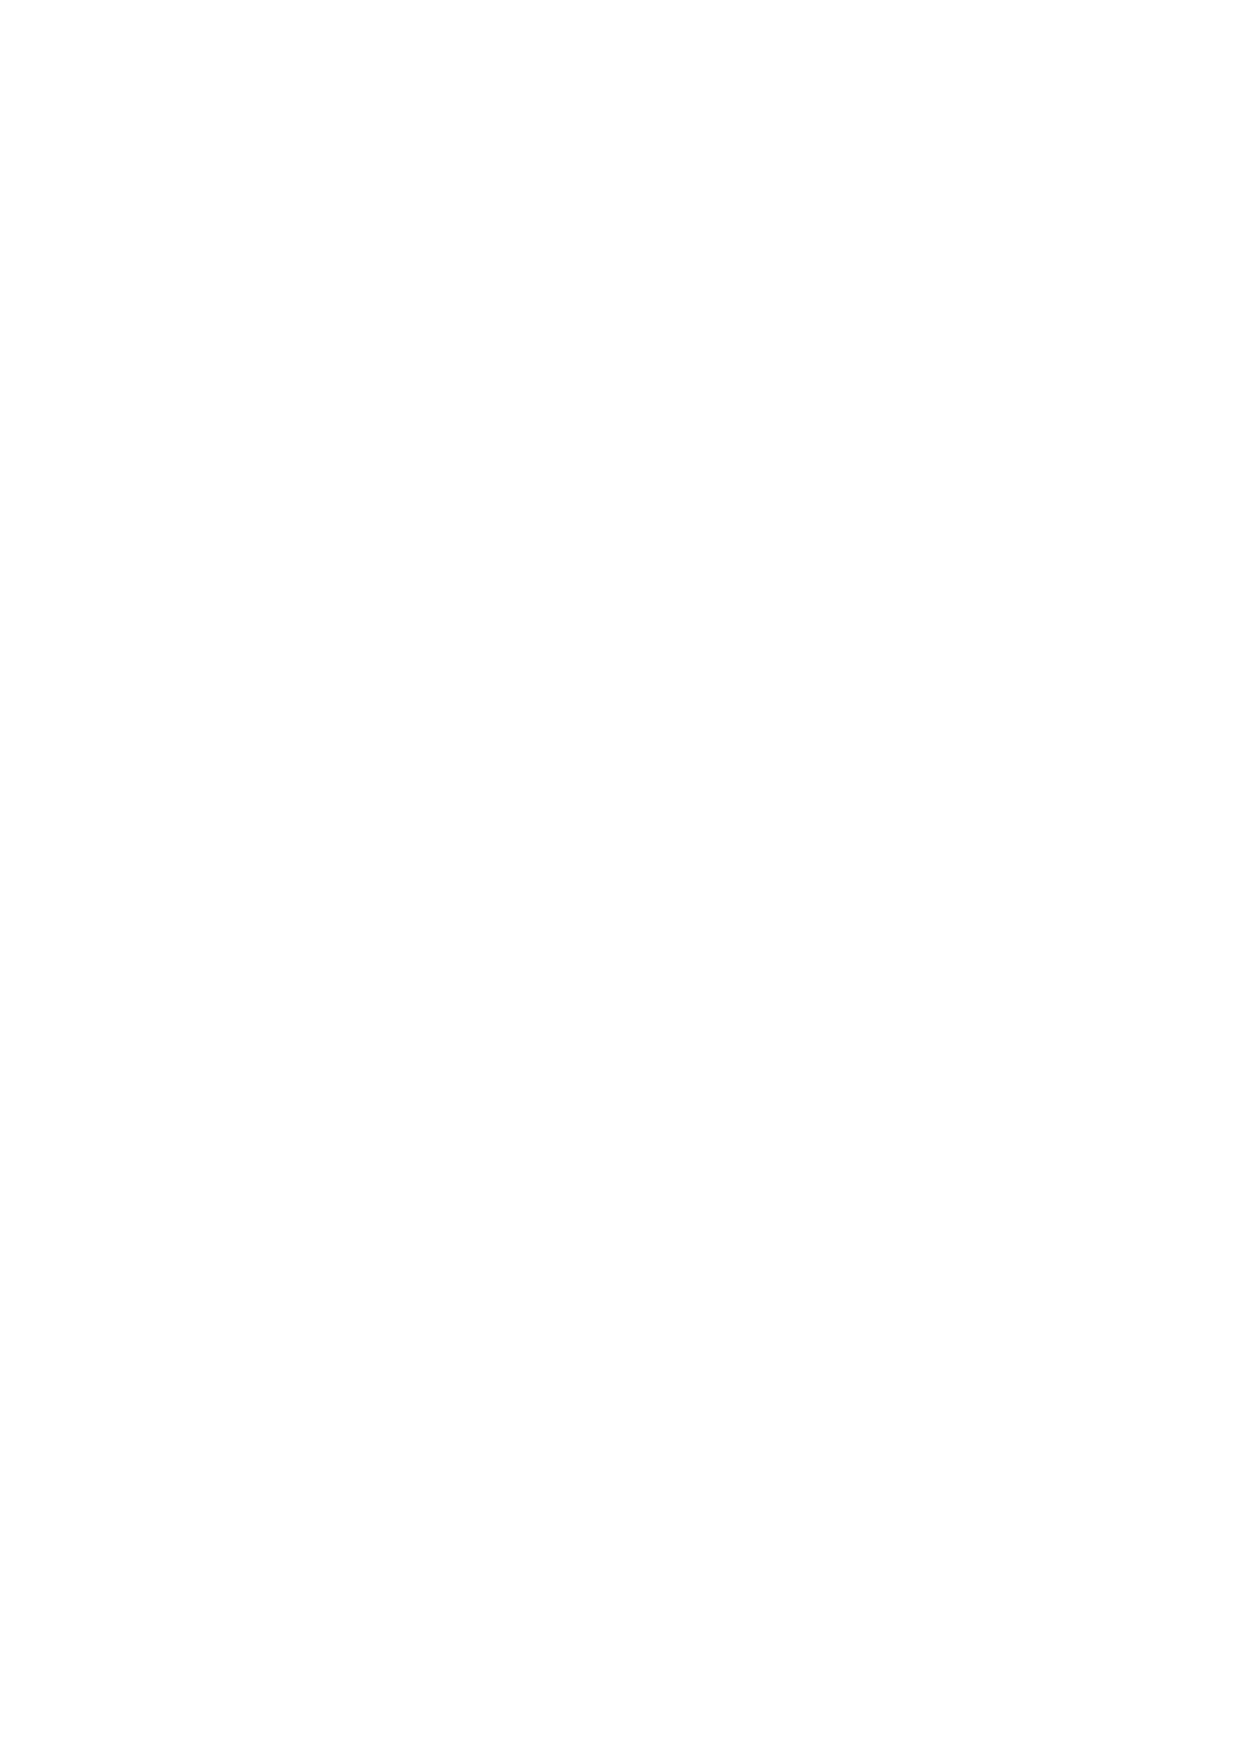
\includegraphics[width=44pt]{class_p_v_node__coll__graph}
\end{center}
\end{figure}
\subsection*{Public Member Functions}
\begin{CompactItemize}
\item 
{\bf PVNode} (const String \&name, SceneNode $\ast$node, Entity $\ast$entity)
\item 
{\bf $\sim$PVNode} ()
\item 
SceneNode $\ast$ {\bf getSceneNode} ()
\item 
Entity $\ast$ {\bf getEntity} ()
\item 
const String \& {\bf getName} ()
\item 
Vector3 {\bf getVelocity} ()
\item 
Vector3 {\bf getAcceleration} ()
\item 
Vector3 {\bf getPosition} ()
\item 
Vector3 {\bf getOrientation} ()
\item 
Vector3 {\bf getNormal} ()
\item 
void {\bf setVelocity} (const Vector3 \&v)
\item 
void {\bf setAcceleration} (const Vector3 \&a)
\item 
void {\bf setPosition} (const Vector3 \&p)
\item 
void {\bf setOrientation} (const Vector3 \&o)
\item 
void {\bf translateNode} (Vector3 trans)
\item 
void {\bf rotateNode} (Direction dir)
\item 
bool {\bf hasAcceleration} ()
\end{CompactItemize}


\subsection{Constructor \& Destructor Documentation}
\index{PVNode@{PVNode}!PVNode@{PVNode}}
\index{PVNode@{PVNode}!PVNode@{PVNode}}
\subsubsection[{PVNode}]{\setlength{\rightskip}{0pt plus 5cm}PVNode::PVNode (const String \& {\em name}, \/  SceneNode $\ast$ {\em node}, \/  Entity $\ast$ {\em entity})}\label{class_p_v_node_b0e321e6d966cf903636415812a3b602}


Constructor. 

\begin{Desc}
\item[Parameters:]
\begin{description}
\item[{\em \&name}]a string. \item[{\em $\ast$node}]an Ogre::SceneNode. \item[{\em $\ast$entity}]an Ogre::Entity. \end{description}
\end{Desc}
\index{PVNode@{PVNode}!$\sim$PVNode@{$\sim$PVNode}}
\index{$\sim$PVNode@{$\sim$PVNode}!PVNode@{PVNode}}
\subsubsection[{$\sim$PVNode}]{\setlength{\rightskip}{0pt plus 5cm}PVNode::$\sim$PVNode ()}\label{class_p_v_node_ba1e77b8f78ad87fdb86038f09d46325}


Destructor. 



\subsection{Member Function Documentation}
\index{PVNode@{PVNode}!getSceneNode@{getSceneNode}}
\index{getSceneNode@{getSceneNode}!PVNode@{PVNode}}
\subsubsection[{getSceneNode}]{\setlength{\rightskip}{0pt plus 5cm}SceneNode$\ast$ PVNode::getSceneNode ()}\label{class_p_v_node_10859a9c5008c31f8a48bb804a21c7e5}


getter for SceneNode. \begin{Desc}
\item[Returns:]m\_\-node a SceneNode pointer. \end{Desc}
\index{PVNode@{PVNode}!getEntity@{getEntity}}
\index{getEntity@{getEntity}!PVNode@{PVNode}}
\subsubsection[{getEntity}]{\setlength{\rightskip}{0pt plus 5cm}Entity$\ast$ PVNode::getEntity ()}\label{class_p_v_node_8a47ecdcd84e3ab1efcd5f7b188421e0}


getter for Entity. \begin{Desc}
\item[Returns:]m\_\-entity an Entity pointer. \end{Desc}
\index{PVNode@{PVNode}!getName@{getName}}
\index{getName@{getName}!PVNode@{PVNode}}
\subsubsection[{getName}]{\setlength{\rightskip}{0pt plus 5cm}const String\& PVNode::getName ()}\label{class_p_v_node_e4504c9d990dab7a5ae388c618d5becb}


getter for PVnode name. \begin{Desc}
\item[Returns:]name a string. \end{Desc}
\index{PVNode@{PVNode}!getVelocity@{getVelocity}}
\index{getVelocity@{getVelocity}!PVNode@{PVNode}}
\subsubsection[{getVelocity}]{\setlength{\rightskip}{0pt plus 5cm}Vector3 PVNode::getVelocity ()}\label{class_p_v_node_998e3f1a2319eff7b2273b0d35125d25}


getter for PVnode velocity. \begin{Desc}
\item[Returns:]m\_\-velocity a Vector3. \end{Desc}
\index{PVNode@{PVNode}!getAcceleration@{getAcceleration}}
\index{getAcceleration@{getAcceleration}!PVNode@{PVNode}}
\subsubsection[{getAcceleration}]{\setlength{\rightskip}{0pt plus 5cm}Vector3 PVNode::getAcceleration ()}\label{class_p_v_node_353bff245238eb8a9c2f113edbf62104}


getter for PVnode acceleration. \begin{Desc}
\item[Returns:]m\_\-acceleration a Vector3. \end{Desc}
\index{PVNode@{PVNode}!getPosition@{getPosition}}
\index{getPosition@{getPosition}!PVNode@{PVNode}}
\subsubsection[{getPosition}]{\setlength{\rightskip}{0pt plus 5cm}Vector3 PVNode::getPosition ()}\label{class_p_v_node_abc34042de0783c6b86084f2a2960edc}


getter for PVnode position. \begin{Desc}
\item[Returns:]m\_\-position a Vector3. \end{Desc}
\index{PVNode@{PVNode}!getOrientation@{getOrientation}}
\index{getOrientation@{getOrientation}!PVNode@{PVNode}}
\subsubsection[{getOrientation}]{\setlength{\rightskip}{0pt plus 5cm}Vector3 PVNode::getOrientation ()}\label{class_p_v_node_ae65e5bd2f9f46737b62ef516d1a36cf}


getter for PVnode orietation. \begin{Desc}
\item[Returns:]m\_\-orientation a Vector3. \end{Desc}
\index{PVNode@{PVNode}!getNormal@{getNormal}}
\index{getNormal@{getNormal}!PVNode@{PVNode}}
\subsubsection[{getNormal}]{\setlength{\rightskip}{0pt plus 5cm}Vector3 PVNode::getNormal ()}\label{class_p_v_node_cbd1e4f9c58205a8ad56d8ff9c855c25}


getter for PVnode normal. \begin{Desc}
\item[Returns:]m\_\-normal a Vector3. \end{Desc}
\index{PVNode@{PVNode}!setVelocity@{setVelocity}}
\index{setVelocity@{setVelocity}!PVNode@{PVNode}}
\subsubsection[{setVelocity}]{\setlength{\rightskip}{0pt plus 5cm}void PVNode::setVelocity (const Vector3 \& {\em v})}\label{class_p_v_node_e19b5a9d0058c23fe0c54aadae0bbe97}


setter for \doxyref{PVNode}{p.}{class_p_v_node} velocity. 

\begin{Desc}
\item[Parameters:]
\begin{description}
\item[{\em \&v}]a Vector3. \end{description}
\end{Desc}
\index{PVNode@{PVNode}!setAcceleration@{setAcceleration}}
\index{setAcceleration@{setAcceleration}!PVNode@{PVNode}}
\subsubsection[{setAcceleration}]{\setlength{\rightskip}{0pt plus 5cm}void PVNode::setAcceleration (const Vector3 \& {\em a})}\label{class_p_v_node_457399ffb92a993b91893dcf0691e237}


setter for \doxyref{PVNode}{p.}{class_p_v_node} acceleration. 

\begin{Desc}
\item[Parameters:]
\begin{description}
\item[{\em \&a}]a Vector3. \end{description}
\end{Desc}
\index{PVNode@{PVNode}!setPosition@{setPosition}}
\index{setPosition@{setPosition}!PVNode@{PVNode}}
\subsubsection[{setPosition}]{\setlength{\rightskip}{0pt plus 5cm}void PVNode::setPosition (const Vector3 \& {\em p})}\label{class_p_v_node_6e97653037d430ce5c9903c7f9d4ecdd}


setter for \doxyref{PVNode}{p.}{class_p_v_node} position. 

\begin{Desc}
\item[Parameters:]
\begin{description}
\item[{\em \&p}]a Vector3. \end{description}
\end{Desc}
\index{PVNode@{PVNode}!setOrientation@{setOrientation}}
\index{setOrientation@{setOrientation}!PVNode@{PVNode}}
\subsubsection[{setOrientation}]{\setlength{\rightskip}{0pt plus 5cm}void PVNode::setOrientation (const Vector3 \& {\em o})}\label{class_p_v_node_74e5faa95f067945e728ad11c04bf31f}


setter for \doxyref{PVNode}{p.}{class_p_v_node} orientation. 

\begin{Desc}
\item[Parameters:]
\begin{description}
\item[{\em \&o}]a Vector3. \end{description}
\end{Desc}
\index{PVNode@{PVNode}!translateNode@{translateNode}}
\index{translateNode@{translateNode}!PVNode@{PVNode}}
\subsubsection[{translateNode}]{\setlength{\rightskip}{0pt plus 5cm}void PVNode::translateNode (Vector3 {\em trans})}\label{class_p_v_node_19695ff7c8e2783f7c7e50762d612741}


translate a PVnode. 

\begin{Desc}
\item[Parameters:]
\begin{description}
\item[{\em trans}]a Vector3. \end{description}
\end{Desc}
\index{PVNode@{PVNode}!rotateNode@{rotateNode}}
\index{rotateNode@{rotateNode}!PVNode@{PVNode}}
\subsubsection[{rotateNode}]{\setlength{\rightskip}{0pt plus 5cm}void PVNode::rotateNode (Direction {\em dir})}\label{class_p_v_node_e5d02f656efde63f5127f7b98561f9f2}


rotates a PVnode in a direction. 

\begin{Desc}
\item[Parameters:]
\begin{description}
\item[{\em dir}]a PVNode::Direction. \end{description}
\end{Desc}
\index{PVNode@{PVNode}!hasAcceleration@{hasAcceleration}}
\index{hasAcceleration@{hasAcceleration}!PVNode@{PVNode}}
\subsubsection[{hasAcceleration}]{\setlength{\rightskip}{0pt plus 5cm}bool PVNode::hasAcceleration ()}\label{class_p_v_node_ffd742f192b5080e10c8f5a250e02d5d}


checks if \doxyref{PVNode}{p.}{class_p_v_node} has acceleration. 

\begin{Desc}
\item[Returns:]true if \doxyref{PVNode}{p.}{class_p_v_node} has an acceleration != 0. \end{Desc}


The documentation for this class was generated from the following files:\begin{CompactItemize}
\item 
PVNode.h\item 
PVNode.cpp\end{CompactItemize}

\section{PVPhysics Class Reference}
\label{class_p_v_physics}\index{PVPhysics@{PVPhysics}}
Collaboration diagram for PVPhysics:\nopagebreak
\begin{figure}[H]
\begin{center}
\leavevmode
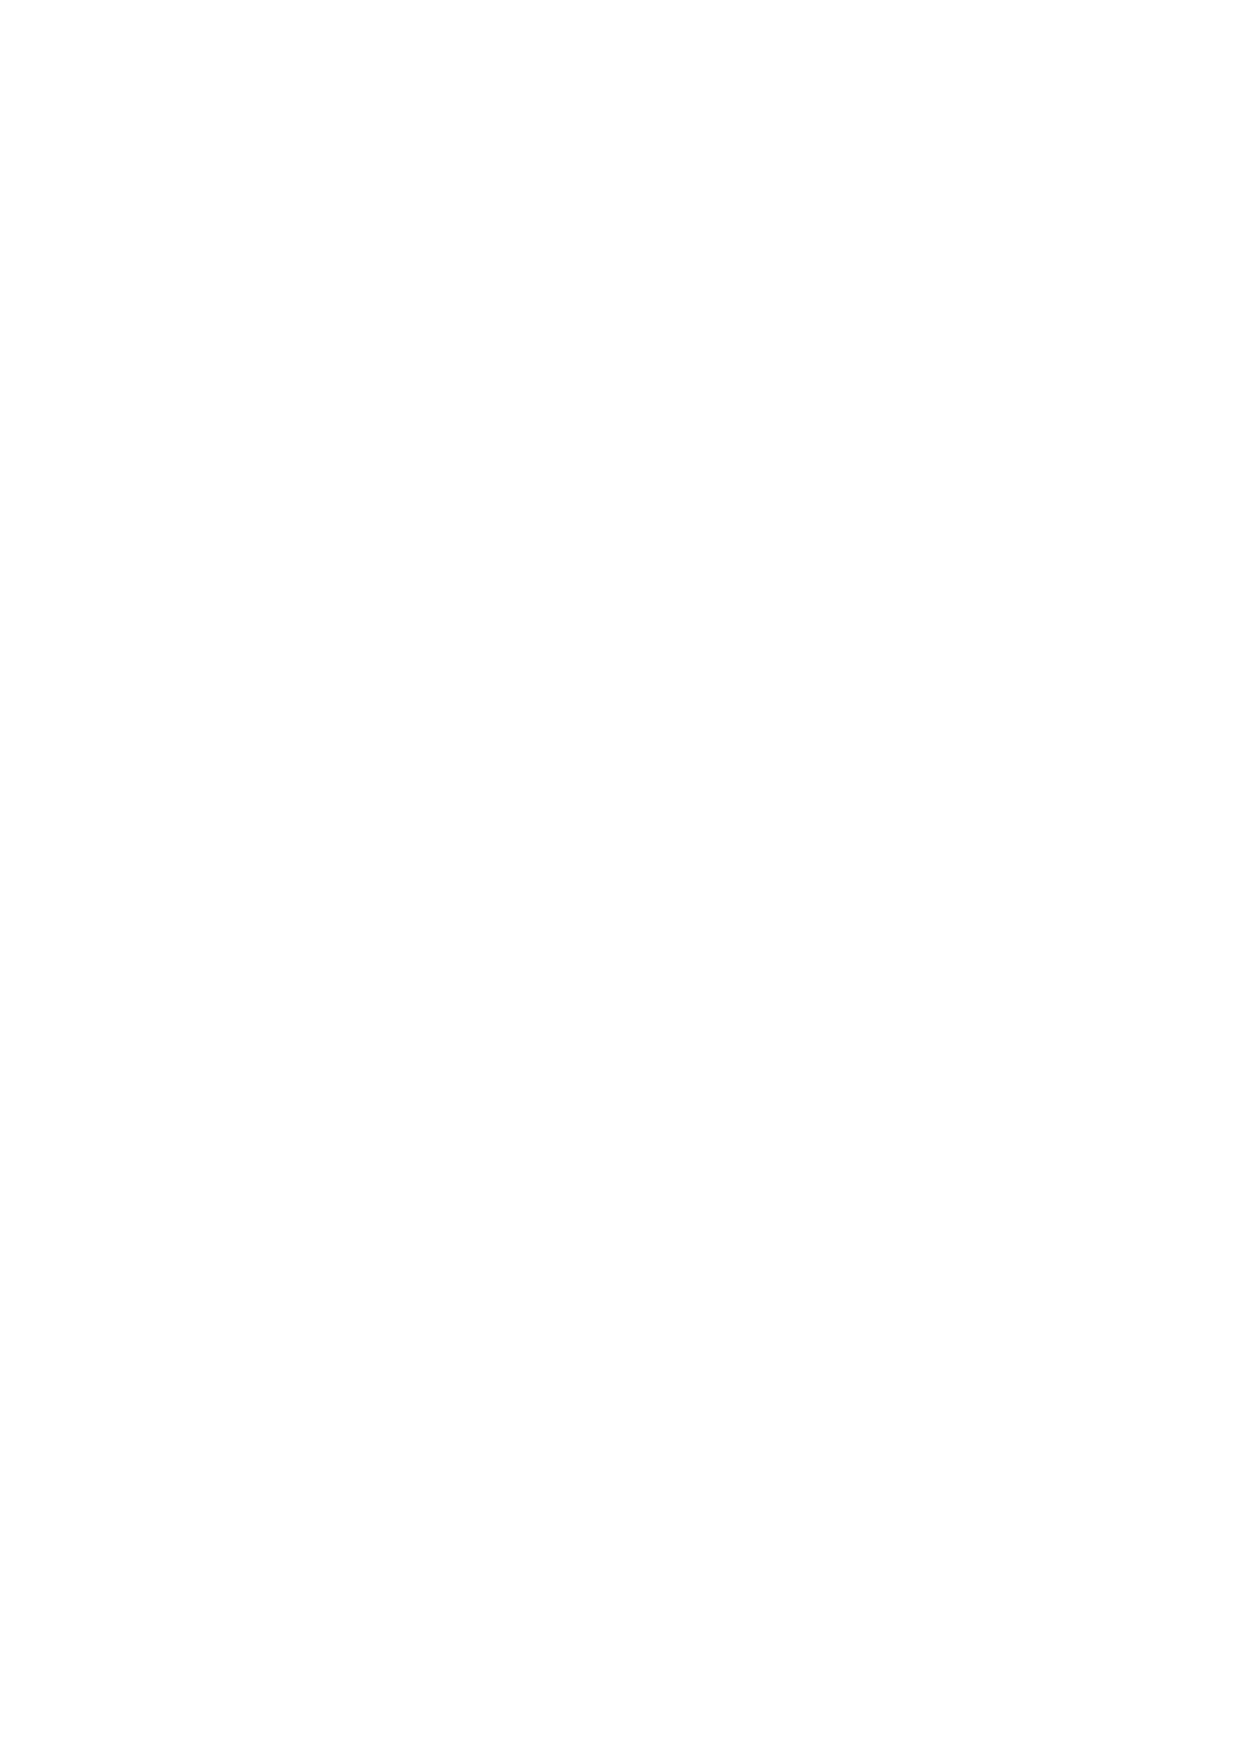
\includegraphics[width=44pt]{class_p_v_physics__coll__graph}
\end{center}
\end{figure}
\subsection*{Public Member Functions}
\begin{CompactItemize}
\item 
{\bf PVPhysics} ()
\item 
{\bf $\sim$PVPhysics} ()
\item 
void {\bf simulate} (std::map$<$ std::string, {\bf PVNode} $\ast$ $>$ \&objectMap, std::vector$<$ {\bf PVNode} $\ast$ $>$ \&balls, int numberOfFlyingBalls, float time)
\item 
void {\bf move} ({\bf PVNode} $\ast$ball, float time)
\item 
void {\bf collisionDetection} (std::map$<$ std::string, {\bf PVNode} $\ast$ $>$ \&objectMap, std::vector$<$ {\bf PVNode} $\ast$ $>$ \&balls, int numberOfFlyingBalls)
\item 
void {\bf collisionWithArena} ({\bf PVNode} $\ast$arena, {\bf PVNode} $\ast$ball)
\item 
void {\bf collisionWithWall} ({\bf PVNode} $\ast$wall, {\bf PVNode} $\ast$ball)
\item 
void {\bf collisionWithCannon} ({\bf PVNode} $\ast$kanone, {\bf PVNode} $\ast$ball)
\item 
void {\bf collisionWithBall} ({\bf PVNode} $\ast$ball1, {\bf PVNode} $\ast$ball2)
\item 
void {\bf collisionWithPillar} ({\bf PVNode} $\ast$pillar, {\bf PVNode} $\ast$ball)
\item 
void {\bf handleCollision} ({\bf PVNode} $\ast$node, {\bf PVNode} $\ast$ball)
\item 
void {\bf handleCollisionWithGround} ({\bf PVNode} $\ast$ground, {\bf PVNode} $\ast$ball)
\item 
void {\bf handleCollisionWithBall} ({\bf PVNode} $\ast$ball1, {\bf PVNode} $\ast$ball2)
\end{CompactItemize}


\subsection{Constructor \& Destructor Documentation}
\index{PVPhysics@{PVPhysics}!PVPhysics@{PVPhysics}}
\index{PVPhysics@{PVPhysics}!PVPhysics@{PVPhysics}}
\subsubsection[{PVPhysics}]{\setlength{\rightskip}{0pt plus 5cm}PVPhysics::PVPhysics ()}\label{class_p_v_physics_aed6e907849a824d51cc2ddd1ab946d7}


Constructor. 

\index{PVPhysics@{PVPhysics}!$\sim$PVPhysics@{$\sim$PVPhysics}}
\index{$\sim$PVPhysics@{$\sim$PVPhysics}!PVPhysics@{PVPhysics}}
\subsubsection[{$\sim$PVPhysics}]{\setlength{\rightskip}{0pt plus 5cm}PVPhysics::$\sim$PVPhysics ()}\label{class_p_v_physics_d1b6443d26383106cb3322671974d48e}


Destructor. 



\subsection{Member Function Documentation}
\index{PVPhysics@{PVPhysics}!simulate@{simulate}}
\index{simulate@{simulate}!PVPhysics@{PVPhysics}}
\subsubsection[{simulate}]{\setlength{\rightskip}{0pt plus 5cm}void PVPhysics::simulate (std::map$<$ std::string, {\bf PVNode} $\ast$ $>$ \& {\em objectMap}, \/  std::vector$<$ {\bf PVNode} $\ast$ $>$ \& {\em balls}, \/  int {\em numberOfFlyingBalls}, \/  float {\em time})}\label{class_p_v_physics_d12e7af8e342acdf42f83d5f1e88dc14}


simulate function which calls move function and collision detection. 

\begin{Desc}
\item[Parameters:]
\begin{description}
\item[{\em objectMap}]map with objects. \item[{\em numberOfFlyingBalls}]current sooted balls. \item[{\em time}]delta time elapsed since last frame in seconds. \end{description}
\end{Desc}
\index{PVPhysics@{PVPhysics}!move@{move}}
\index{move@{move}!PVPhysics@{PVPhysics}}
\subsubsection[{move}]{\setlength{\rightskip}{0pt plus 5cm}void PVPhysics::move ({\bf PVNode} $\ast$ {\em ball}, \/  float {\em time})}\label{class_p_v_physics_ef493f065afc2637f704ec9fd5cb8754}


function for shooting a ball. 

\begin{Desc}
\item[Parameters:]
\begin{description}
\item[{\em ball}]a PVnode. \item[{\em time}]a float for the time since last frame. \end{description}
\end{Desc}
\index{PVPhysics@{PVPhysics}!collisionDetection@{collisionDetection}}
\index{collisionDetection@{collisionDetection}!PVPhysics@{PVPhysics}}
\subsubsection[{collisionDetection}]{\setlength{\rightskip}{0pt plus 5cm}void PVPhysics::collisionDetection (std::map$<$ std::string, {\bf PVNode} $\ast$ $>$ \& {\em objectMap}, \/  std::vector$<$ {\bf PVNode} $\ast$ $>$ \& {\em balls}, \/  int {\em numberOfFlyingBalls})}\label{class_p_v_physics_e56c458a7f62c983e2ab5f903bee9478}


function for calling the particular collision detection function for each node type. 

\begin{Desc}
\item[Parameters:]
\begin{description}
\item[{\em objectMap}]map with all scene nodes. \item[{\em balls}]vector with all balls. \end{description}
\end{Desc}
\index{PVPhysics@{PVPhysics}!collisionWithArena@{collisionWithArena}}
\index{collisionWithArena@{collisionWithArena}!PVPhysics@{PVPhysics}}
\subsubsection[{collisionWithArena}]{\setlength{\rightskip}{0pt plus 5cm}void PVPhysics::collisionWithArena ({\bf PVNode} $\ast$ {\em arena}, \/  {\bf PVNode} $\ast$ {\em ball})}\label{class_p_v_physics_35f87bc90c8aae2772d79523bcb4bf77}


detects collision between arena and a ball. 

\begin{Desc}
\item[Parameters:]
\begin{description}
\item[{\em $\ast$arena}]scene node. \item[{\em $\ast$ball}]\end{description}
\end{Desc}
\index{PVPhysics@{PVPhysics}!collisionWithWall@{collisionWithWall}}
\index{collisionWithWall@{collisionWithWall}!PVPhysics@{PVPhysics}}
\subsubsection[{collisionWithWall}]{\setlength{\rightskip}{0pt plus 5cm}void PVPhysics::collisionWithWall ({\bf PVNode} $\ast$ {\em wall}, \/  {\bf PVNode} $\ast$ {\em ball})}\label{class_p_v_physics_7e07bd0171a431a2ccf4e542348d0820}


detects collision between wall and a ball. 

\begin{Desc}
\item[Parameters:]
\begin{description}
\item[{\em $\ast$wall}]scene node. \item[{\em $\ast$ball}]\end{description}
\end{Desc}
\index{PVPhysics@{PVPhysics}!collisionWithCannon@{collisionWithCannon}}
\index{collisionWithCannon@{collisionWithCannon}!PVPhysics@{PVPhysics}}
\subsubsection[{collisionWithCannon}]{\setlength{\rightskip}{0pt plus 5cm}void PVPhysics::collisionWithCannon ({\bf PVNode} $\ast$ {\em kanone}, \/  {\bf PVNode} $\ast$ {\em ball})}\label{class_p_v_physics_967d8b19b11aef754591e6d9336ecfbe}


detects collision between arena and a ball. 

\begin{Desc}
\item[Parameters:]
\begin{description}
\item[{\em $\ast$kanone}]scene node \item[{\em $\ast$ball}]\end{description}
\end{Desc}
\index{PVPhysics@{PVPhysics}!collisionWithBall@{collisionWithBall}}
\index{collisionWithBall@{collisionWithBall}!PVPhysics@{PVPhysics}}
\subsubsection[{collisionWithBall}]{\setlength{\rightskip}{0pt plus 5cm}void PVPhysics::collisionWithBall ({\bf PVNode} $\ast$ {\em ball1}, \/  {\bf PVNode} $\ast$ {\em ball2})}\label{class_p_v_physics_d55e28ab26fc818faf43231a3368294c}


detects collisionbetween balls. 

\begin{Desc}
\item[Parameters:]
\begin{description}
\item[{\em $\ast$ball1}]scene node. \item[{\em $\ast$ball2}]\end{description}
\end{Desc}
\index{PVPhysics@{PVPhysics}!collisionWithPillar@{collisionWithPillar}}
\index{collisionWithPillar@{collisionWithPillar}!PVPhysics@{PVPhysics}}
\subsubsection[{collisionWithPillar}]{\setlength{\rightskip}{0pt plus 5cm}void PVPhysics::collisionWithPillar ({\bf PVNode} $\ast$ {\em pillar}, \/  {\bf PVNode} $\ast$ {\em ball})}\label{class_p_v_physics_2e69d5b10735bec201d92e9206e618cb}


detects collisionbetween pillar and a ball. 

\begin{Desc}
\item[Parameters:]
\begin{description}
\item[{\em $\ast$pillar}]scene node. \item[{\em $\ast$ball}]\end{description}
\end{Desc}
\index{PVPhysics@{PVPhysics}!handleCollision@{handleCollision}}
\index{handleCollision@{handleCollision}!PVPhysics@{PVPhysics}}
\subsubsection[{handleCollision}]{\setlength{\rightskip}{0pt plus 5cm}void PVPhysics::handleCollision ({\bf PVNode} $\ast$ {\em node}, \/  {\bf PVNode} $\ast$ {\em ball})}\label{class_p_v_physics_43833f09fa8abc6114290d9161d14bb5}


handles collision between a ball and a scene node. 

\begin{Desc}
\item[Parameters:]
\begin{description}
\item[{\em node}]a scene node. \item[{\em ball}]a ball. \end{description}
\end{Desc}
\index{PVPhysics@{PVPhysics}!handleCollisionWithGround@{handleCollisionWithGround}}
\index{handleCollisionWithGround@{handleCollisionWithGround}!PVPhysics@{PVPhysics}}
\subsubsection[{handleCollisionWithGround}]{\setlength{\rightskip}{0pt plus 5cm}void PVPhysics::handleCollisionWithGround ({\bf PVNode} $\ast$ {\em ground}, \/  {\bf PVNode} $\ast$ {\em ball})}\label{class_p_v_physics_5c037709dbad69c82c4fa0437a0f6c69}


handles collision between ground and a ball. 

\begin{Desc}
\item[Parameters:]
\begin{description}
\item[{\em ground}]a scene node. \item[{\em ball}]a ball. \end{description}
\end{Desc}
\index{PVPhysics@{PVPhysics}!handleCollisionWithBall@{handleCollisionWithBall}}
\index{handleCollisionWithBall@{handleCollisionWithBall}!PVPhysics@{PVPhysics}}
\subsubsection[{handleCollisionWithBall}]{\setlength{\rightskip}{0pt plus 5cm}void PVPhysics::handleCollisionWithBall ({\bf PVNode} $\ast$ {\em ball1}, \/  {\bf PVNode} $\ast$ {\em ball2})}\label{class_p_v_physics_b33b7fee9e0d4eada11603880f2d4a40}


handles collision between balls. 

\begin{Desc}
\item[Parameters:]
\begin{description}
\item[{\em ball1}]first ball. \item[{\em ball2}]second ball. \end{description}
\end{Desc}


The documentation for this class was generated from the following files:\begin{CompactItemize}
\item 
PVPhysics.h\item 
PVPhysics.cpp\end{CompactItemize}

\section{PVTimer Class Reference}
\label{class_p_v_timer}\index{PVTimer@{PVTimer}}
Collaboration diagram for PVTimer:\nopagebreak
\begin{figure}[H]
\begin{center}
\leavevmode
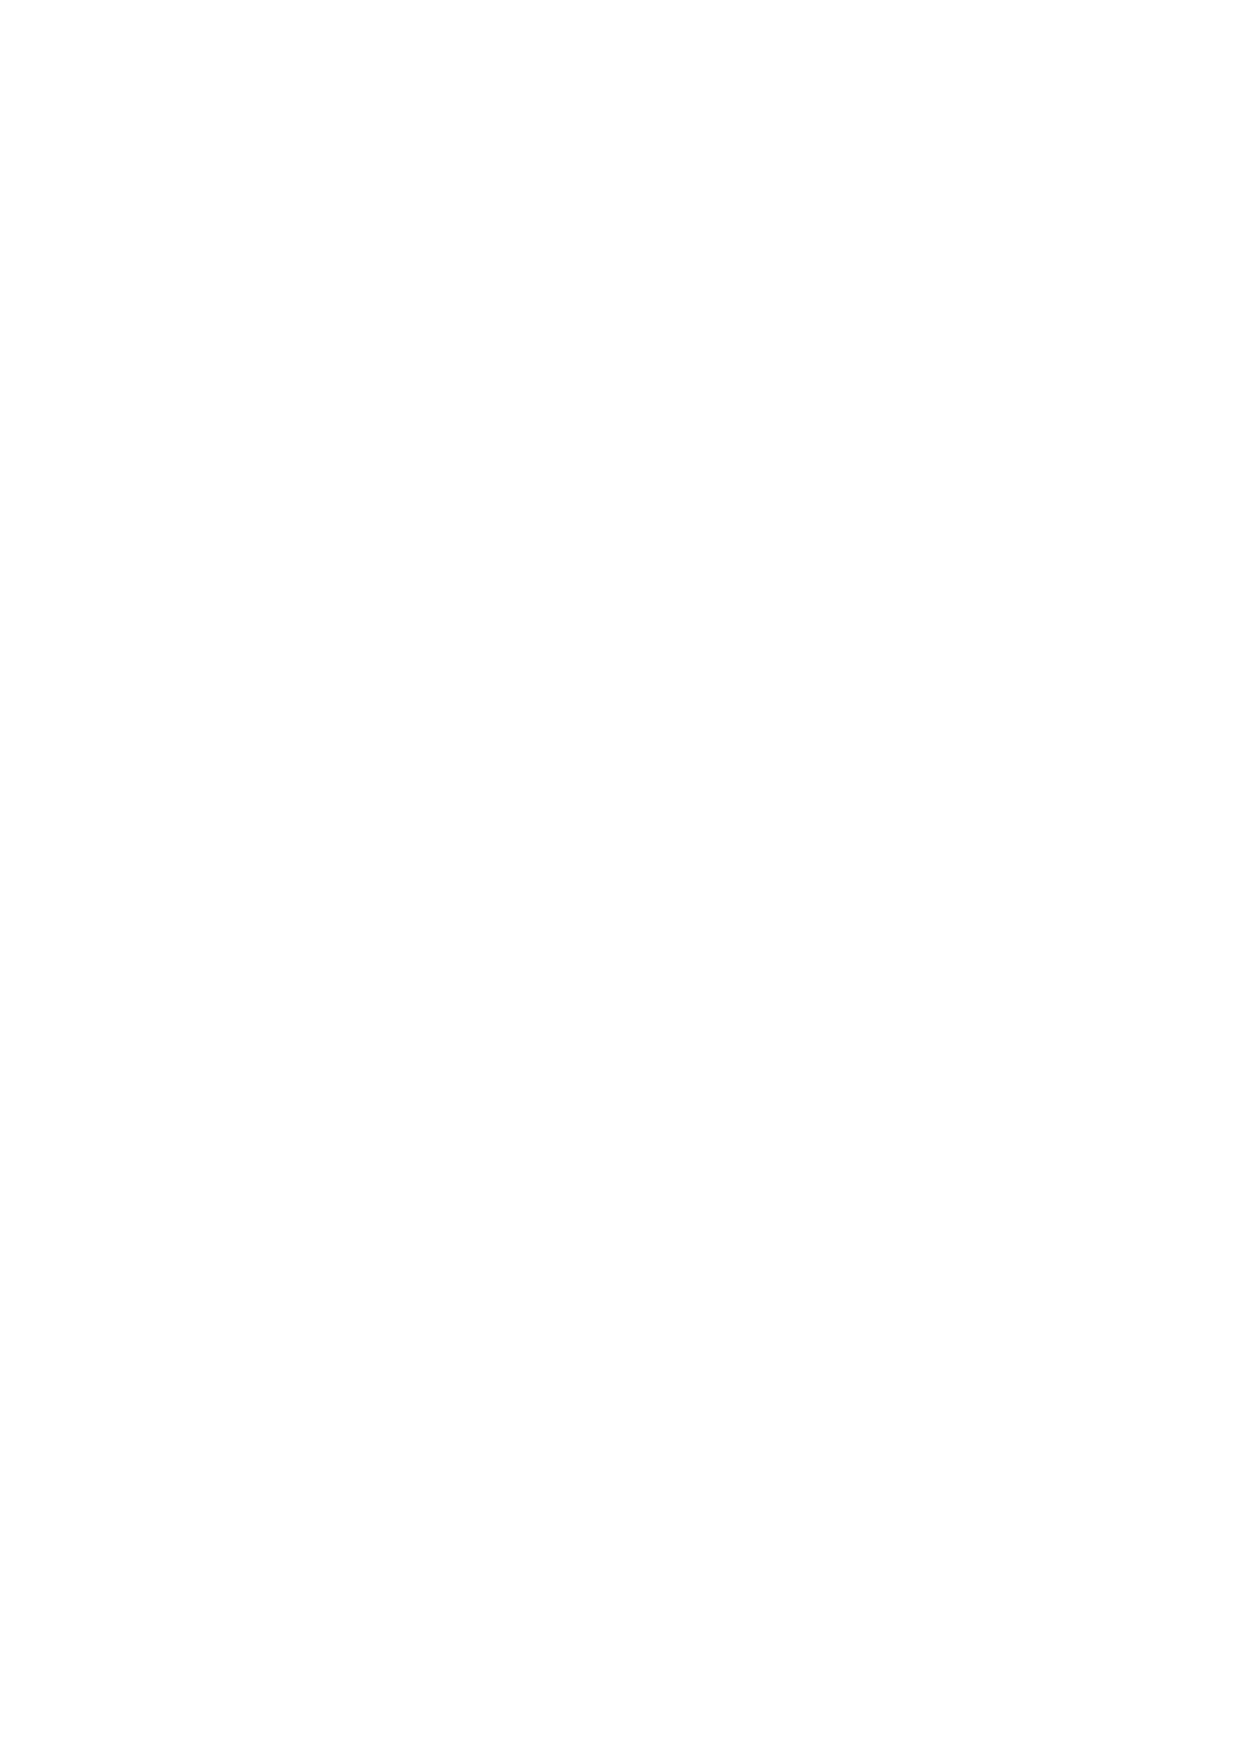
\includegraphics[width=44pt]{class_p_v_timer__coll__graph}
\end{center}
\end{figure}
\subsection*{Public Member Functions}
\begin{CompactItemize}
\item 
double {\bf messureTime} ()
\item 
double {\bf diffClockMs} (clock\_\-t t1, clock\_\-t t2)
\end{CompactItemize}
\subsection*{Static Public Member Functions}
\begin{CompactItemize}
\item 
static {\bf PVTimer} \& {\bf getInstance} ()
\end{CompactItemize}


\subsection{Member Function Documentation}
\index{PVTimer@{PVTimer}!getInstance@{getInstance}}
\index{getInstance@{getInstance}!PVTimer@{PVTimer}}
\subsubsection[{getInstance}]{\setlength{\rightskip}{0pt plus 5cm}static {\bf PVTimer}\& PVTimer::getInstance ()\hspace{0.3cm}{\tt  [static]}}\label{class_p_v_timer_c0f313309b0ea2324458fc2f277aa83b}


\index{PVTimer@{PVTimer}!messureTime@{messureTime}}
\index{messureTime@{messureTime}!PVTimer@{PVTimer}}
\subsubsection[{messureTime}]{\setlength{\rightskip}{0pt plus 5cm}double PVTimer::messureTime ()}\label{class_p_v_timer_28722001b6635db85c03f8c2bcdd5073}


\index{PVTimer@{PVTimer}!diffClockMs@{diffClockMs}}
\index{diffClockMs@{diffClockMs}!PVTimer@{PVTimer}}
\subsubsection[{diffClockMs}]{\setlength{\rightskip}{0pt plus 5cm}double PVTimer::diffClockMs (clock\_\-t {\em t1}, \/  clock\_\-t {\em t2})}\label{class_p_v_timer_bddabecd73093c64294a30aa3144c077}




The documentation for this class was generated from the following files:\begin{CompactItemize}
\item 
PVTimer.h\item 
PVTimer.cpp\end{CompactItemize}

\printindex
\end{document}
